% Kompilasi dengan XeLaTeX: latexmk -xelatex Laporan_Evaluasi_Model_Kelompok_SDT.tex
% Format mengikuti dokumen Microsoft Word: Times New Roman 12 pt, persamaan gaya Equation Word
% (Cambria Math, tiap persamaan rata tengah, kata dalam rumus tegak),
% tabel gaya "Table Grid" (paket tabularray), tanpa pemenggalan kata, jarak antarparagraf 8 pt tanpa indentasi.
\documentclass[12pt,a4paper]{article}

\usepackage[a4paper,margin=2.54cm]{geometry}
\usepackage{amsmath}
\usepackage{fontspec}
\usepackage{unicode-math}
\setmainfont{Times New Roman}[Ligatures=NoCommon]
\setmonofont{Courier New}[Ligatures=NoCommon]
\setmathfont{Cambria Math}
\usepackage[indonesian]{babel}

\usepackage{graphicx}
\usepackage{array}
\usepackage{tabularray}
\usepackage[labelsep=period,font=normalsize,labelfont=bf,justification=centering,skip=6pt]{caption}
\usepackage{enumitem}
\usepackage{titlesec}
\usepackage[section]{placeins}
\usepackage{xurl}
\usepackage[hidelinks]{hyperref}

% Paragraf gaya Word: tanpa indentasi baris pertama, jarak 8 pt setelah paragraf.
% Jarak baris 14,5 pt pada 12 pt setara spasi "multiple 1,08" Word untuk Times New Roman.
\setlength{\parindent}{0pt}
\setlength{\parskip}{8pt}
\emergencystretch=3em
\hfuzz=1.5pt

% Persamaan gaya Equation Word: tiap persamaan satu baris rata tengah (gather*), jarak antarbaris
% persamaan 8 pt seperti jarak paragraf, kata dalam rumus memakai \symup (Cambria Math tegak).
\setlength{\jot}{8pt}

% Judul bagian: Times New Roman 12 pt tebal, hitam, bernomor "1." dan "1.1".
\titleformat{\section}{\normalfont\bfseries}{\thesection.}{0.5em}{}
\titleformat{\subsection}{\normalfont\bfseries}{\thesubsection}{0.5em}{}
\titlespacing*{\section}{0pt}{12pt}{0pt}
\titlespacing*{\subsection}{0pt}{8pt}{0pt}

% Daftar berpoin gaya Word: poin di 0,63 cm, teks di 1,27 cm, tanpa jarak antarbutir.
\setlist[itemize]{label=\textbullet,leftmargin=1.27cm,labelindent=0.63cm,labelsep=*,align=left,itemsep=0pt,parsep=0pt,topsep=0pt}
\setlist[enumerate]{leftmargin=1.27cm,labelindent=0.63cm,labelsep=*,align=left,itemsep=0pt,parsep=0pt,topsep=0pt}

% Tabel gaya "Table Grid": garis 0,5 pt di semua sel, padding sel 0,19 cm, header tebal rata tengah.
% Perataan isi: teks rata kiri, angka rata kanan (desimal seragam per kolom), kode pendek rata tengah.
\NewTblrEnviron{grid}
\SetTblrInner[grid]{hlines={0.5pt}, vlines={0.5pt}, colsep=0.19cm, rowsep=1.5pt,
  cells={valign=m}, row{1}={font=\bfseries, halign=c}}

\graphicspath{{../figures/}{./}}
\newcommand{\kode}[1]{\texttt{#1}}

\begin{document}
\hyphenpenalty=10000
\exhyphenpenalty=10000

% ------------------------------------------------------------------ SAMPUL
\begin{titlepage}
\centering
\vspace*{0.5cm}
{\fontsize{14}{17}\selectfont\bfseries TUGAS KELOMPOK\par}
\vspace{0.4cm}
{\fontsize{16}{20}\selectfont\bfseries EVALUASI MODEL DATA SCIENCE\par}
\vspace{0.3cm}
{\fontsize{14}{17}\selectfont\bfseries Studi Kasus Pengawasan Truk ODOL\par}
(\textit{Over Dimension Over Load})\par
\vspace{1.2cm}


\includegraphics[height=4.5cm]{logo_ugm.png}\par
\vspace{1.2cm}
\textbf{Anggota Kelompok}\par
\vspace{0.3cm}
\begin{grid}{width=0.85\linewidth, colspec={Q[c,1.2cm] X[l] Q[c,4.6cm]}, row{1}={halign=c}}
No & Nama & NIM \\
1 & Hafidz Rizqullah Prasetya & 24/535493/SV/24243 \\
2 & Pralambang Bhayangkara Yhudanto & 24/536223/SV/24414 \\
3 & Alfiz Desta Ariant Permana & 24/543220/SV/25173 \\
4 & Danny Setiawan & 24/541304/SV/24894 \\
\end{grid}

\vfill
Mata Kuliah Sains Data Terapan (SVPL261506)\par
Dosen: Dr.~Muhammad Fakhrurrifqi dan Anindita Suryarasmi, Ph.D.\par
\vspace{0.6cm}
{\bfseries SARJANA TERAPAN TEKNOLOGI REKAYASA PERANGKAT LUNAK\par
DEPARTEMEN TEKNIK ELEKTRO DAN INFORMATIKA\par
SEKOLAH VOKASI UNIVERSITAS GADJAH MADA\par
2026\par}
\end{titlepage}

% ------------------------------------------------------------------ 1
\section{Pendahuluan}

Tugas ini meminta kelompok membuat contoh kasus berisi nilai aktual dan hasil prediksi model, lalu menghitung evaluasinya untuk empat jenis model: regresi, clustering, klasifikasi tiga kelas, dan deteksi objek. Keempat bagian memakai satu tema, yaitu pengawasan truk ODOL: truk yang dimensi atau muatannya melebihi batas izin. Tema ini melanjutkan tugas sebelumnya, ketika kelompok melatih model YOLO11n untuk mendeteksi truk ODOL.

\begin{table}[htbp]
\centering
\caption{Ringkasan contoh kasus tiap bagian}
\label{tab:kasus}
\begin{grid}{width=\linewidth, colspec={Q[l,2.7cm] X[l] Q[l,3.4cm]}, row{1}={halign=c}}
Bagian & Kasus & Data \\
Regresi & Sensor \textit{Weigh-in-Motion} (WIM) memperkirakan berat kotor truk saat melaju, dibandingkan dengan jembatan timbang statis & 10 truk (karangan) \\
Clustering & Pengelompokan truk berdasarkan rasio dimensi dan rasio muatan terhadap batas izin & 12 truk (karangan) \\
Klasifikasi & Penentuan status truk: \kode{normal}, \kode{overload}, atau \kode{overdimension} & 30 truk (karangan) \\
Deteksi objek & Model YOLO11n mendeteksi \kode{roda}, \kode{truk\_normal}, dan \kode{truk\_odol} & 5 gambar \textit{test} asli \\
\end{grid}
\end{table}

Setiap metrik dihitung manual, lalu dicocokkan dengan pustaka \kode{scikit-learn} dan \kode{ultralytics}. Seluruh perhitungan ada di notebook \kode{evaluasi\_model.ipynb}, dan semua hasil manual sama dengan hasil pustaka.

% ------------------------------------------------------------------ 2
\section{Evaluasi Regresi}

\subsection{Kasus dan Data}
Sensor WIM di jalan arteri memperkirakan berat kotor truk tanpa truk harus berhenti. Nilai aktual $y$ diambil dari jembatan timbang statis, dan nilai prediksi $\hat y$ dari WIM. Error tiap truk adalah $e_i = y_i - \hat y_i$. Rata-rata berat aktual $\bar y = 22{,}91$~ton.

\begin{table}[htbp]
\centering
\caption{Data regresi dan tabel bantu perhitungan (satuan ton, kecuali kolom persen)}
\label{tab:regresi}
\begin{grid}{width=\linewidth, colspec={Q[c,1.3cm] X[r] X[r] X[r] X[r] X[r] X[r] X[r] X[r]}, row{1}={halign=c}}
Truk & $y$ & $\hat y$ & $e$ & $|e|$ & $e^2$ & $|e|/y$ (\%) & $|y-\bar y|$ & $(y-\bar y)^2$ \\
T01 & 8,2  & 8,9  & $-0{,}7$ & 0,7 & 0,49 & 8,54 & 14,71 & 216,38 \\
T02 & 12,5 & 11,8 & 0,7      & 0,7 & 0,49 & 5,60 & 10,41 & 108,37 \\
T03 & 15,0 & 16,1 & $-1{,}1$ & 1,1 & 1,21 & 7,33 & 7,91  & 62,57 \\
T04 & 18,4 & 17,6 & 0,8      & 0,8 & 0,64 & 4,35 & 4,51  & 20,34 \\
T05 & 21,7 & 23,0 & $-1{,}3$ & 1,3 & 1,69 & 5,99 & 1,21  & 1,46 \\
T06 & 24,3 & 23,5 & 0,8      & 0,8 & 0,64 & 3,29 & 1,39  & 1,93 \\
T07 & 26,8 & 28,9 & $-2{,}1$ & 2,1 & 4,41 & 7,84 & 3,89  & 15,13 \\
T08 & 30,5 & 29,4 & 1,1      & 1,1 & 1,21 & 3,61 & 7,59  & 57,61 \\
T09 & 33,1 & 35,8 & $-2{,}7$ & 2,7 & 7,29 & 8,16 & 10,19 & 103,84 \\
T10 & 38,6 & 36,2 & 2,4      & 2,4 & 5,76 & 6,22 & 15,69 & 246,18 \\
$\Sigma$ & & & & 13,70 & 23,83 & 60,92 & 77,50 & 833,81 \\
\end{grid}
\end{table}

\subsection{Perhitungan}
Dengan $n = 10$:
\begin{gather*}
\symup{MAE}  = \frac{1}{n}\sum |e_i| = \frac{13{,}70}{10} = 1{,}370 \,\symup{ton}\\
\symup{MSE}  = \frac{1}{n}\sum e_i^2 = \frac{23{,}83}{10} = 2{,}383 \,\symup{ton}^2\\
\symup{RMSE} = \sqrt{\symup{MSE}} = \sqrt{2{,}383} = 1{,}544 \,\symup{ton}\\
R^2 = 1 - \frac{\sum e_i^2}{\sum (y_i-\bar y)^2} = 1 - \frac{23{,}83}{833{,}81} = 0{,}9714\\
\symup{MAPE} = \frac{1}{n}\sum \frac{|e_i|}{y_i}\times 100\% = \frac{60{,}92\%}{10} = 6{,}09\%\\
\symup{MPE} = \frac{1}{n}\sum \frac{e_i}{y_i}\times 100\% = \frac{-14{,}79\%}{10} = -1{,}48\%\\
\symup{RAE} = \frac{\sum |e_i|}{\sum |y_i-\bar y|} = \frac{13{,}70}{77{,}50} = 0{,}1768\\
\symup{RSE} = \frac{\sum e_i^2}{\sum (y_i-\bar y)^2} = \frac{23{,}83}{833{,}81} = 0{,}0286
\end{gather*}

\begin{figure}[htbp]
\centering
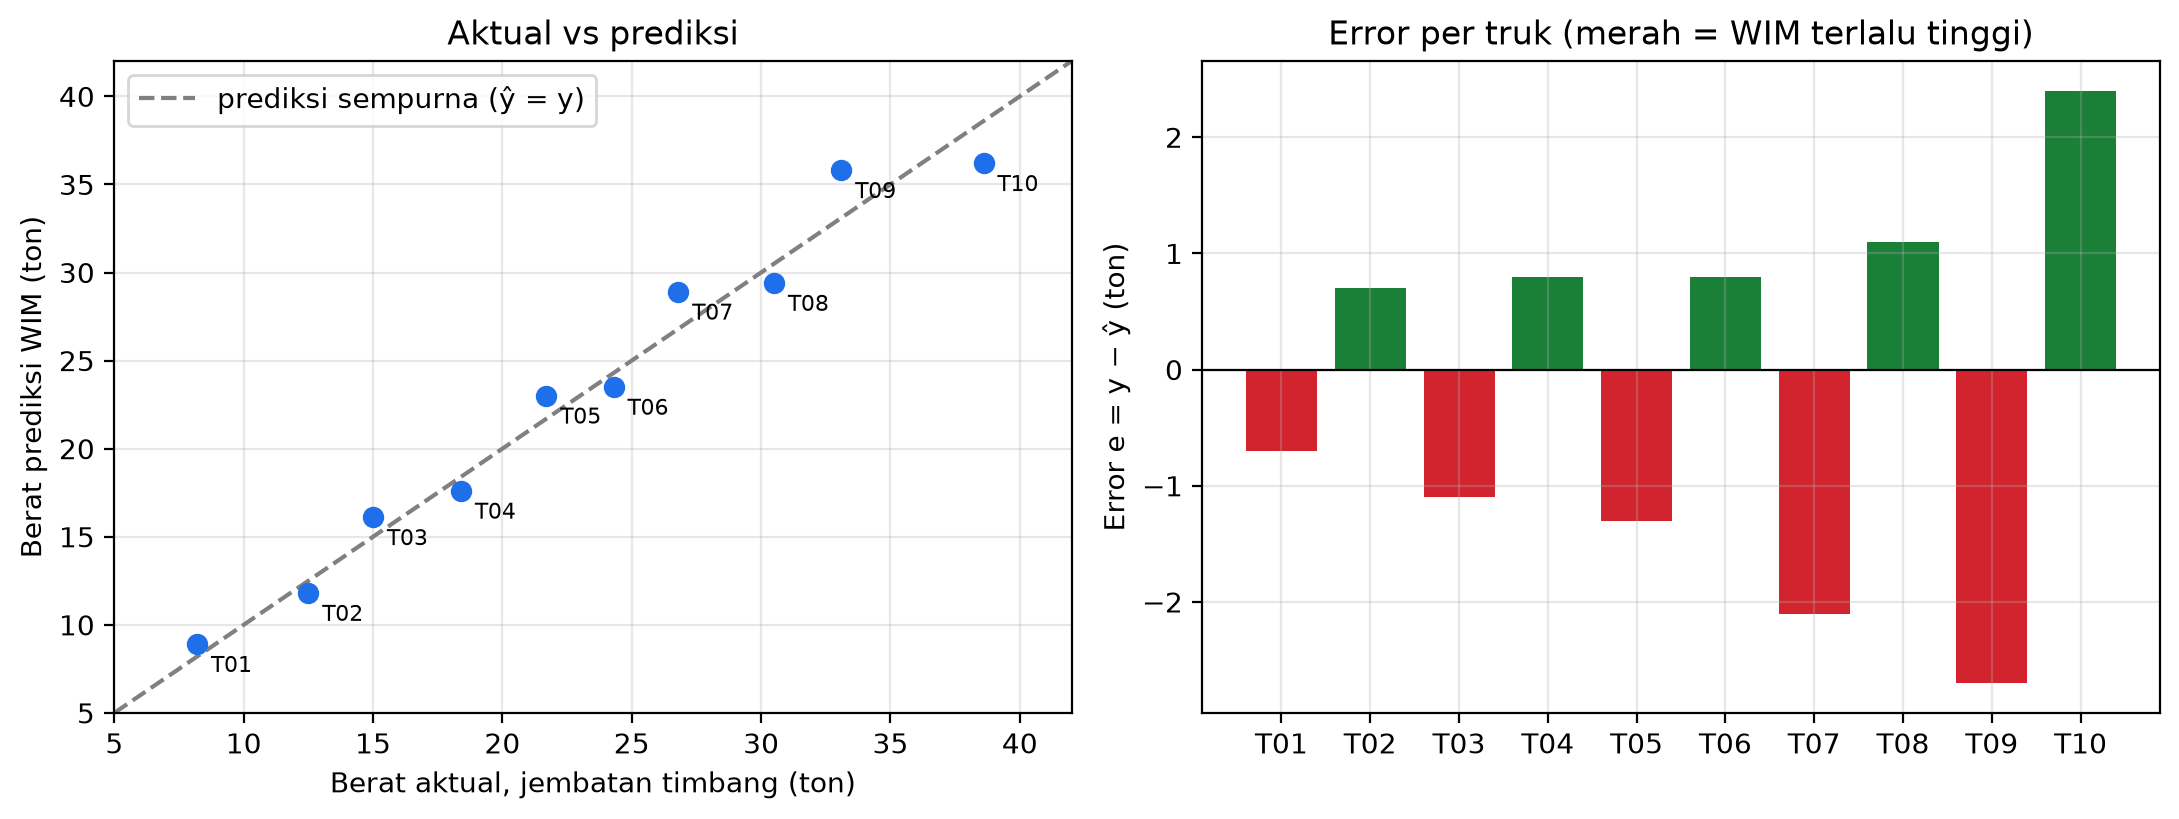
\includegraphics[width=\linewidth]{regresi_aktual_vs_prediksi.png}
\caption{Kiri: berat aktual terhadap prediksi WIM; garis putus-putus adalah prediksi sempurna. Kanan: error tiap truk; batang merah berarti WIM melebihkan berat}
\label{fig:regresi}
\end{figure}

\subsection{Interpretasi}
\begin{itemize}
\item MAE 1,37~ton dan MAPE 6,09\% berarti perkiraan WIM rata-rata meleset sekitar 1,4~ton atau 6\% dari berat sebenarnya.
\item RMSE (1,54~ton) lebih besar daripada MAE karena beberapa error besar, yaitu T09 (2,7~ton) dan T10 (2,4~ton), dihukum lebih berat oleh pengkuadratan.
\item $R^2 = 0{,}971$: WIM menjelaskan sekitar 97\% variasi berat truk, sehingga urutan berat truk ditebak dengan sangat baik.
\item MPE bernilai negatif ($-1{,}48\%$), artinya WIM sedikit cenderung melebihkan berat. Untuk penindakan ODOL, kecenderungan ini membuat truk yang sebenarnya patuh bisa tercatat \textit{overload}. WIM lebih cocok dipakai sebagai penyaring awal sebelum truk ditimbang ulang secara statis.
\end{itemize}

% ------------------------------------------------------------------ 3
\section{Evaluasi Clustering}

\subsection{Kasus dan Data}
Dua belas truk dikelompokkan tanpa label berdasarkan dua fitur: rasio dimensi bak terhadap batas izin ($x_1$) dan rasio muatan terhadap Jumlah Berat yang Diizinkan atau JBI ($x_2$). Nilai 100\% berarti tepat di batas. Kedua fitur bersatuan persen, sehingga jarak Euclidean bisa dipakai tanpa normalisasi. Clustering tidak memiliki label aktual, jadi yang dinilai adalah kualitas kelompok yang terbentuk.

\subsection{K-Means Manual (k = 3)}
Centroid awal diambil dari truk C01 $(88, 82)$, C05 $(98, 128)$, dan C09 $(125, 145)$. Pada iterasi pertama setiap truk masuk ke centroid terdekat, sehingga terbentuk kelompok \{C01--C04\}, \{C05--C08\}, dan \{C09--C12\}. Centroid kemudian diperbarui menjadi rata-rata anggotanya. Pada iterasi kedua keanggotaan tidak berubah, sehingga algoritma konvergen. Centroid akhir: $c_0 = (91{,}25;\ 88{,}25)$, $c_1 = (98{,}25;\ 128{,}75)$, $c_2 = (126{,}25;\ 148{,}25)$.

\begin{table}[htbp]
\centering
\caption{Data clustering, hasil cluster, dan nilai silhouette tiap truk}
\label{tab:clustering}
\begin{grid}{width=\linewidth, colspec={Q[c,1.3cm] X[r] X[r] Q[c,1.6cm] X[r] X[r] X[r] X[r]}, row{1}={halign=c}}
Truk & $x_1$ (\%) & $x_2$ (\%) & Cluster & $\lVert x - c\rVert^2$ & $a(i)$ & $b(i)$ & $s(i)$ \\
C01 & 88  & 82  & 0 & 49,63  & 10,05 & 48,28 & 0,792 \\
C02 & 92  & 90  & 0 & 3,63   & 6,44  & 39,71 & 0,838 \\
C03 & 95  & 86  & 0 & 19,13  & 7,79  & 43,17 & 0,820 \\
C04 & 90  & 95  & 0 & 47,13  & 9,61  & 35,43 & 0,729 \\
C05 & 98  & 128 & 1 & 0,63   & 12,40 & 35,33 & 0,649 \\
C06 & 94  & 135 & 1 & 57,13  & 12,99 & 35,55 & 0,635 \\
C07 & 104 & 112 & 1 & 313,63 & 23,68 & 27,15 & 0,128 \\
C08 & 97  & 140 & 1 & 128,13 & 15,58 & 31,22 & 0,501 \\
C09 & 125 & 145 & 2 & 12,13  & 10,41 & 33,01 & 0,685 \\
C10 & 132 & 160 & 2 & 171,13 & 18,18 & 47,01 & 0,613 \\
C11 & 120 & 150 & 2 & 42,13  & 12,37 & 31,86 & 0,612 \\
C12 & 128 & 138 & 2 & 108,13 & 14,80 & 33,05 & 0,552 \\
\end{grid}
\end{table}

\subsection{Inertia}
Inertia adalah jumlah kuadrat jarak setiap truk ke centroid cluster-nya:
\[
\symup{Inertia} = \sum_{i} \lVert x_i - c_{k(i)} \rVert^2 = 119{,}5 + 499{,}5 + 333{,}5 = 952{,}5
\]
Ketiga suku adalah jumlah kolom $\lVert x - c\rVert^2$ per cluster pada Tabel~\ref{tab:clustering}.

\subsection{Silhouette}
Untuk tiap truk, $a(i)$ adalah rata-rata jarak ke anggota lain di cluster yang sama, $b(i)$ adalah rata-rata jarak ke anggota cluster terdekat lainnya, dan
\[
s(i) = \frac{b(i) - a(i)}{\max\bigl(a(i), b(i)\bigr)}.
\]
Contoh untuk C07: $a = 23{,}68$, $b = 27{,}15$ (cluster 0), sehingga $s = (27{,}15 - 23{,}68)/27{,}15 = 0{,}128$. Rata-rata seluruh $s(i)$ pada Tabel~\ref{tab:clustering} memberikan \textbf{Silhouette} $= 0{,}6294$. Rata-rata per cluster: 0,795 (cluster 0), 0,478 (cluster 1), dan 0,616 (cluster 2).

\subsection{Davies-Bouldin Index}
Sebaran cluster $s_i$ adalah rata-rata jarak anggota ke centroid-nya: $s_0 = 5{,}047$, $s_1 = 9{,}344$, $s_2 = 8{,}363$. Jarak antarcentroid: $M_{01} = 41{,}10$, $M_{02} = 69{,}46$, $M_{12} = 34{,}12$. Rasio kemiripan $R_{ij} = (s_i + s_j)/M_{ij}$:
\begin{gather*}
R_{01} = \frac{5{,}047 + 9{,}344}{41{,}10} = 0{,}350\\
R_{02} = \frac{5{,}047 + 8{,}363}{69{,}46} = 0{,}193\\
R_{12} = \frac{9{,}344 + 8{,}363}{34{,}12} = 0{,}519
\end{gather*}
Nilai $D_i = \max_{j\neq i} R_{ij}$ adalah $D_0 = 0{,}350$, $D_1 = 0{,}519$, $D_2 = 0{,}519$, sehingga
\[
\symup{DBI} = \frac{0{,}350 + 0{,}519 + 0{,}519}{3} = 0{,}4627.
\]

\begin{figure}[htbp]
\centering
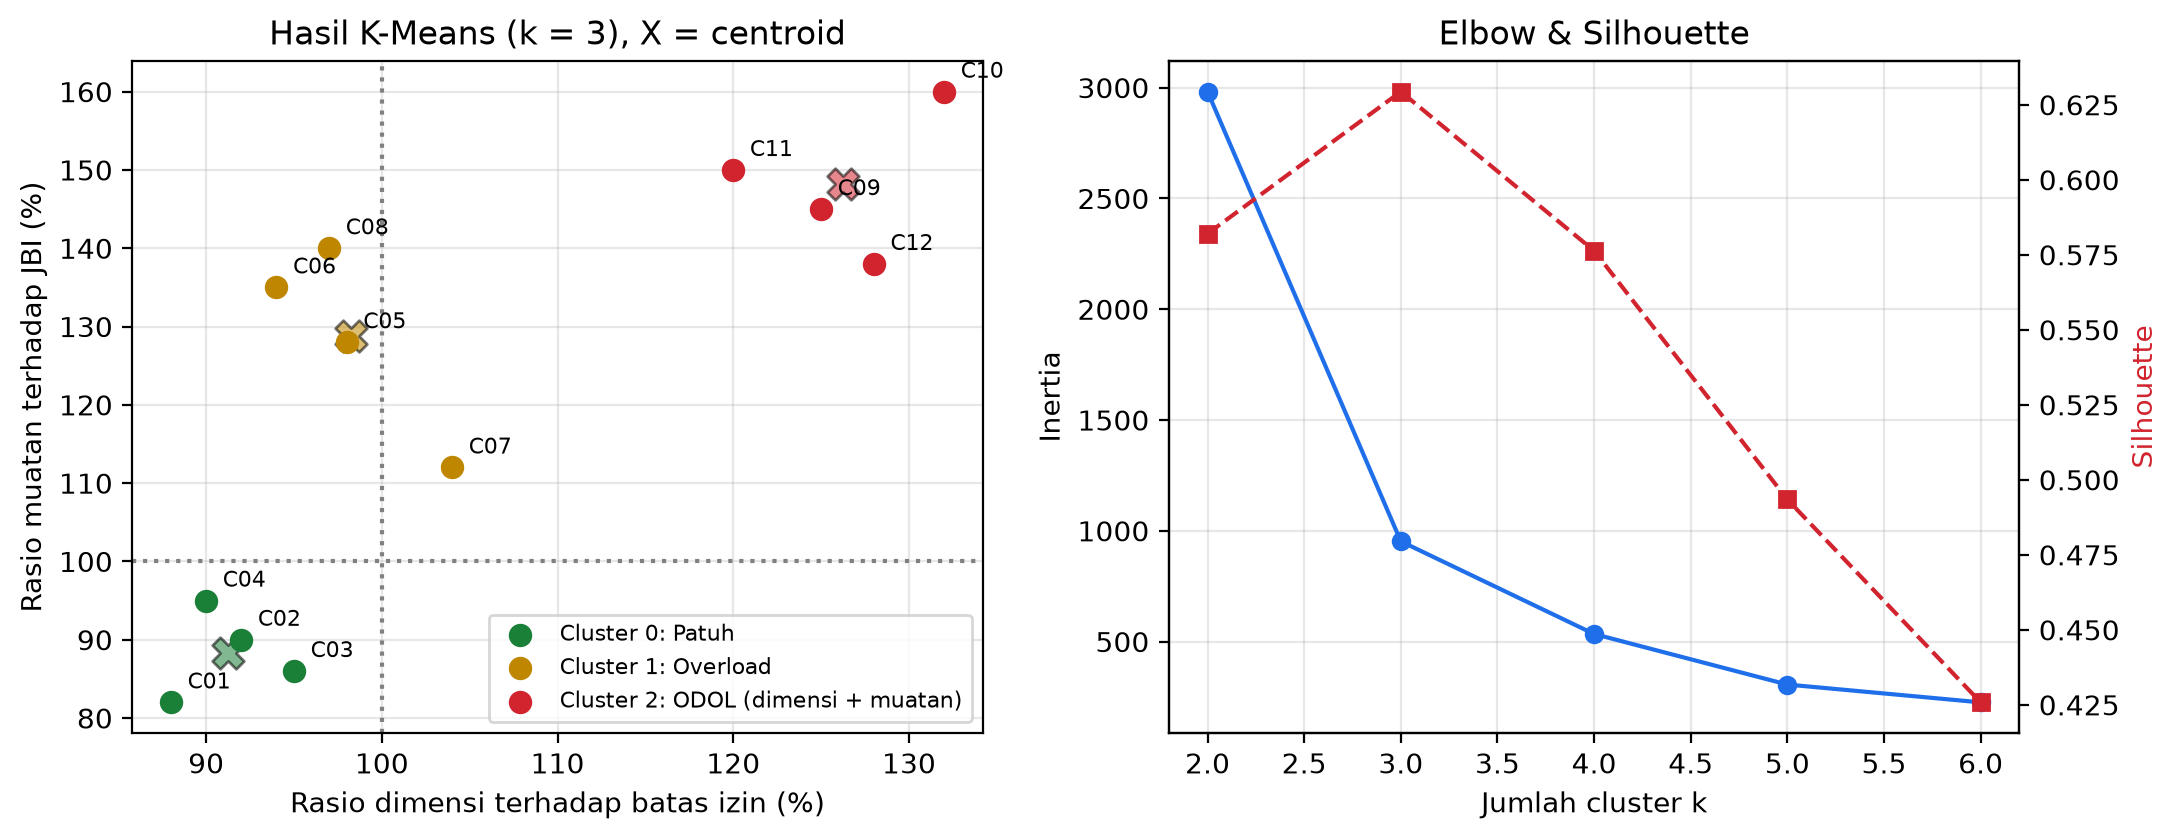
\includegraphics[width=\linewidth]{clustering_kmeans.png}
\caption{Kiri: hasil K-Means $k = 3$, tanda X adalah centroid dan garis titik-titik adalah batas 100\%. Kanan: inertia dan silhouette untuk $k = 2$ sampai 6}
\label{fig:clustering}
\end{figure}

\begin{table}[htbp]
\centering
\caption{Perbandingan jumlah cluster $k$ (K-Means \kode{scikit-learn})}
\label{tab:pilihk}
\begin{grid}{width=\linewidth, colspec={Q[c,1.5cm] X[r] X[r] X[r]}, row{1}={halign=c}}
k & Inertia & Silhouette & Davies-Bouldin \\
2 & 2981,94 & 0,5820 & 0,5108 \\
3 & 952,50  & 0,6294 & 0,4627 \\
4 & 534,33  & 0,5763 & 0,3063 \\
5 & 306,17  & 0,4934 & 0,2780 \\
6 & 225,83  & 0,4258 & 0,2631 \\
\end{grid}
\end{table}

\subsection{Interpretasi}
\begin{itemize}
\item Silhouette 0,63 menunjukkan cluster cukup kompak dan terpisah. C07 memiliki $s(i)$ terkecil (0,128) karena letaknya di antara kelompok patuh dan \textit{overload} dengan rasio muatan 112\%.
\item DBI 0,46 menunjukkan kemiripan antarcluster rendah. Pasangan paling mirip adalah cluster \textit{overload} dan ODOL ($R_{12} = 0{,}519$).
\item Inertia turun tajam dari $k = 2$ ke $k = 3$ (2982 ke 952) lalu melandai, dan silhouette tertinggi juga di $k = 3$. DBI memang terus turun saat $k$ bertambah karena cluster makin kecil, tetapi dua metrik lain sepakat bahwa $k = 3$ adalah pilihan yang wajar.
\item Validasi bisnis: ketiga cluster mudah dijelaskan. Cluster 0 berisi truk \textbf{patuh} (kedua rasio di bawah 100\%), cluster 1 truk \textbf{overload} (muatan melebihi JBI, dimensi wajar), dan cluster 2 truk \textbf{ODOL} (dimensi dan muatan sama-sama melebihi batas). Kelompok ODOL dapat diprioritaskan untuk penindakan dan normalisasi bak.
\end{itemize}

% ------------------------------------------------------------------ 4
\section{Evaluasi Klasifikasi Tiga Kelas}

\subsection{Kasus dan Data}
Sebuah model menentukan status pelanggaran utama tiap truk dari data sensor gerbang: \kode{normal}, \kode{overload} (muatan berlebih), atau \kode{overdimension} (ukuran bak melebihi izin). Status aktual berasal dari pemeriksaan petugas. Data berisi 30 truk dengan komposisi tidak seimbang: 15 \kode{normal}, 9 \kode{overload}, dan 6 \kode{overdimension}. Daftar lengkap per truk ada di \kode{data/klasifikasi\_status\_muatan.csv}.

\begin{table}[htbp]
\centering
\caption{Confusion matrix (baris = aktual, kolom = prediksi)}
\label{tab:cm}
\begin{grid}{width=\linewidth, column{1}={font=\bfseries}, row{5}={font=\bfseries}, colspec={Q[l,3.6cm] X[c] X[c] Q[c,2.9cm] X[c]}, row{1}={halign=c}}
Aktual \textbackslash{} Prediksi & normal & overload & overdimension & Jumlah \\
normal        & \textbf{13} & 2 & 0 & 15 \\
overload      & 2 & \textbf{6} & 1 & 9 \\
overdimension & 1 & 1 & \textbf{4} & 6 \\
Jumlah        & 16 & 9 & 5 & 30 \\
\end{grid}
\end{table}

\subsection{Perhitungan}
Untuk kasus multikelas, TP, FP, FN, dan TN dihitung per kelas dengan cara \textit{one-vs-rest}. TP adalah nilai diagonal kelas tersebut, FP adalah jumlah kolom dikurangi TP, FN adalah jumlah baris dikurangi TP, dan TN adalah sisanya. Contoh untuk kelas \kode{overload}: TP $= 6$, FP $= (2 + 6 + 1) - 6 = 3$, FN $= (2 + 6 + 1) - 6 = 3$, TN $= 30 - 6 - 3 - 3 = 18$, sehingga
\[
\symup{Precision} = \frac{6}{6+3} = 0{,}667, \quad
\symup{Recall} = \frac{6}{6+3} = 0{,}667, \quad
F_1 = \frac{2 \cdot 0{,}667 \cdot 0{,}667}{0{,}667 + 0{,}667} = 0{,}667.
\]

\begin{table}[htbp]
\centering
\caption{Metrik per kelas dan rata-ratanya}
\label{tab:perkelas}
\begin{grid}{width=\linewidth, colspec={Q[l,2.9cm] Q[r,0.65cm] Q[r,0.65cm] Q[r,0.65cm] Q[r,0.65cm] Q[r,1.45cm] X[r] X[r] X[r]}, row{1}={halign=c}}
Kelas & TP & FP & FN & TN & Jumlah & Precision & Recall & $F_1$ \\
normal        & 13 & 3 & 2 & 12 & 15 & 0,8125 & 0,8667 & 0,8387 \\
overload      & 6  & 3 & 3 & 18 & 9  & 0,6667 & 0,6667 & 0,6667 \\
overdimension & 4  & 1 & 2 & 23 & 6  & 0,8000 & 0,6667 & 0,7273 \\
Macro avg     &    &   &   &    & 30 & 0,7597 & 0,7333 & 0,7442 \\
Weighted avg  &    &   &   &    & 30 & 0,7662 & 0,7667 & 0,7648 \\
\end{grid}
\end{table}

\[
\symup{Accuracy} = \frac{13 + 6 + 4}{30} = \frac{23}{30} = 0{,}7667
\]
Rata-rata \textit{macro} adalah rata-rata biasa ketiga kelas, misalnya $F_1^{\symup{macro}} = (0{,}8387 + 0{,}6667 + 0{,}7273)/3 = 0{,}7442$. Rata-rata \textit{weighted} memberi bobot sesuai jumlah data aktual tiap kelas (kolom Jumlah atau \textit{support}).

\begin{figure}[htbp]
\centering
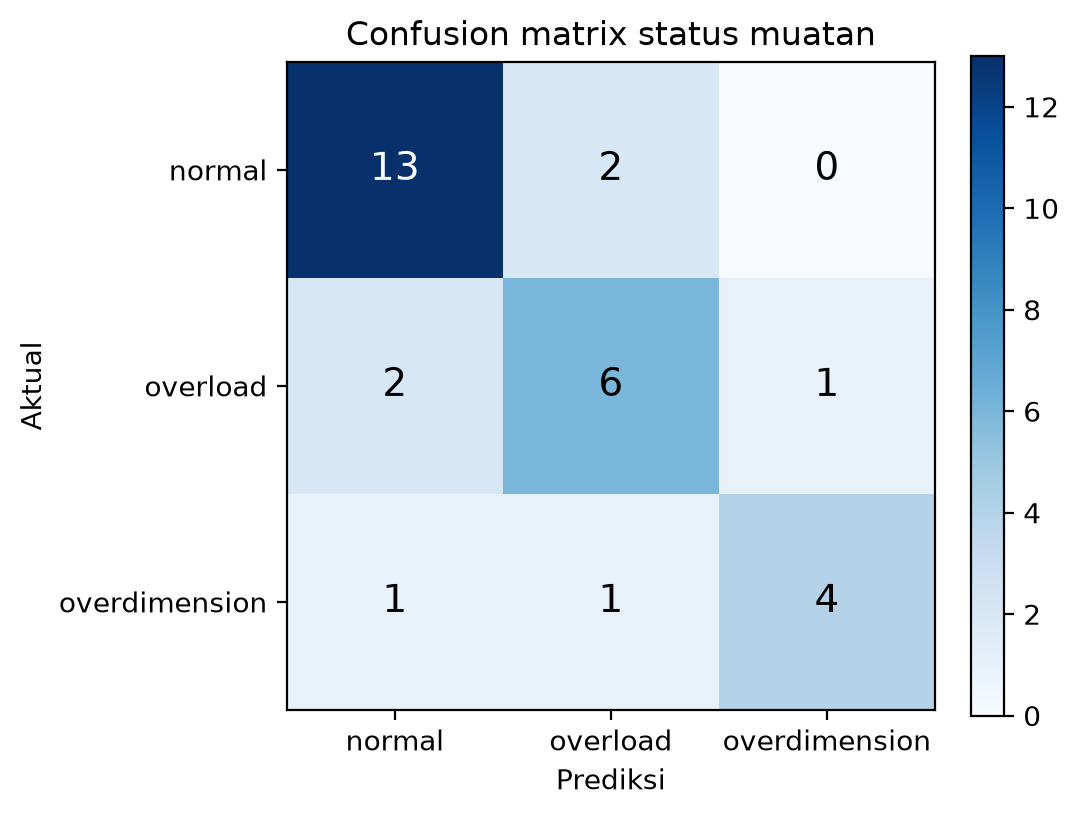
\includegraphics[width=0.55\linewidth]{klasifikasi_confusion_matrix.png}
\caption{Visualisasi confusion matrix status muatan}
\label{fig:cm}
\end{figure}

\subsection{Interpretasi}
\begin{itemize}
\item Accuracy 76,7\% terlihat lumayan, tetapi separuh data adalah truk \kode{normal}. Model yang selalu menebak \kode{normal} saja sudah mencapai accuracy 50\%. Karena itu metrik per kelas dan macro $F_1$ (0,744) memberi gambaran yang lebih jujur.
\item Kelas \kode{normal} paling baik ($F_1 = 0{,}839$). Kelas \kode{overload} paling lemah presisinya: 3 dari 9 truk yang diprediksi \textit{overload} ternyata bukan.
\item Kelas \kode{overdimension} memiliki precision 0,80 tetapi recall hanya 0,67: 2 dari 6 truk \textit{overdimension} lolos (satu dianggap \kode{normal}, satu dianggap \kode{overload}). Dalam pengawasan ODOL kesalahan ini paling berbahaya karena truk yang melanggar dibiarkan lewat, sehingga recall kelas pelanggaran sebaiknya diprioritaskan.
\end{itemize}

% ------------------------------------------------------------------ 5
\section{Evaluasi Deteksi Objek}

\subsection{Kasus dan Data}
Model YOLO11n hasil tugas sebelumnya mendeteksi tiga kelas: \kode{roda}, \kode{truk\_normal}, dan \kode{truk\_odol}. Diambil lima gambar dari \textit{test set}: dua yang terdeteksi sempurna (0001 dan 0002) dan tiga yang mengandung kesalahan (0010, 0029, 0100). Kotak \textit{ground truth} (GT) berasal dari anotasi Roboflow, sedangkan prediksi berasal dari model dengan ambang \textit{confidence} 0,25. Totalnya ada 16 kotak GT dan 18 kotak prediksi.

\begin{figure}[htbp]
\centering
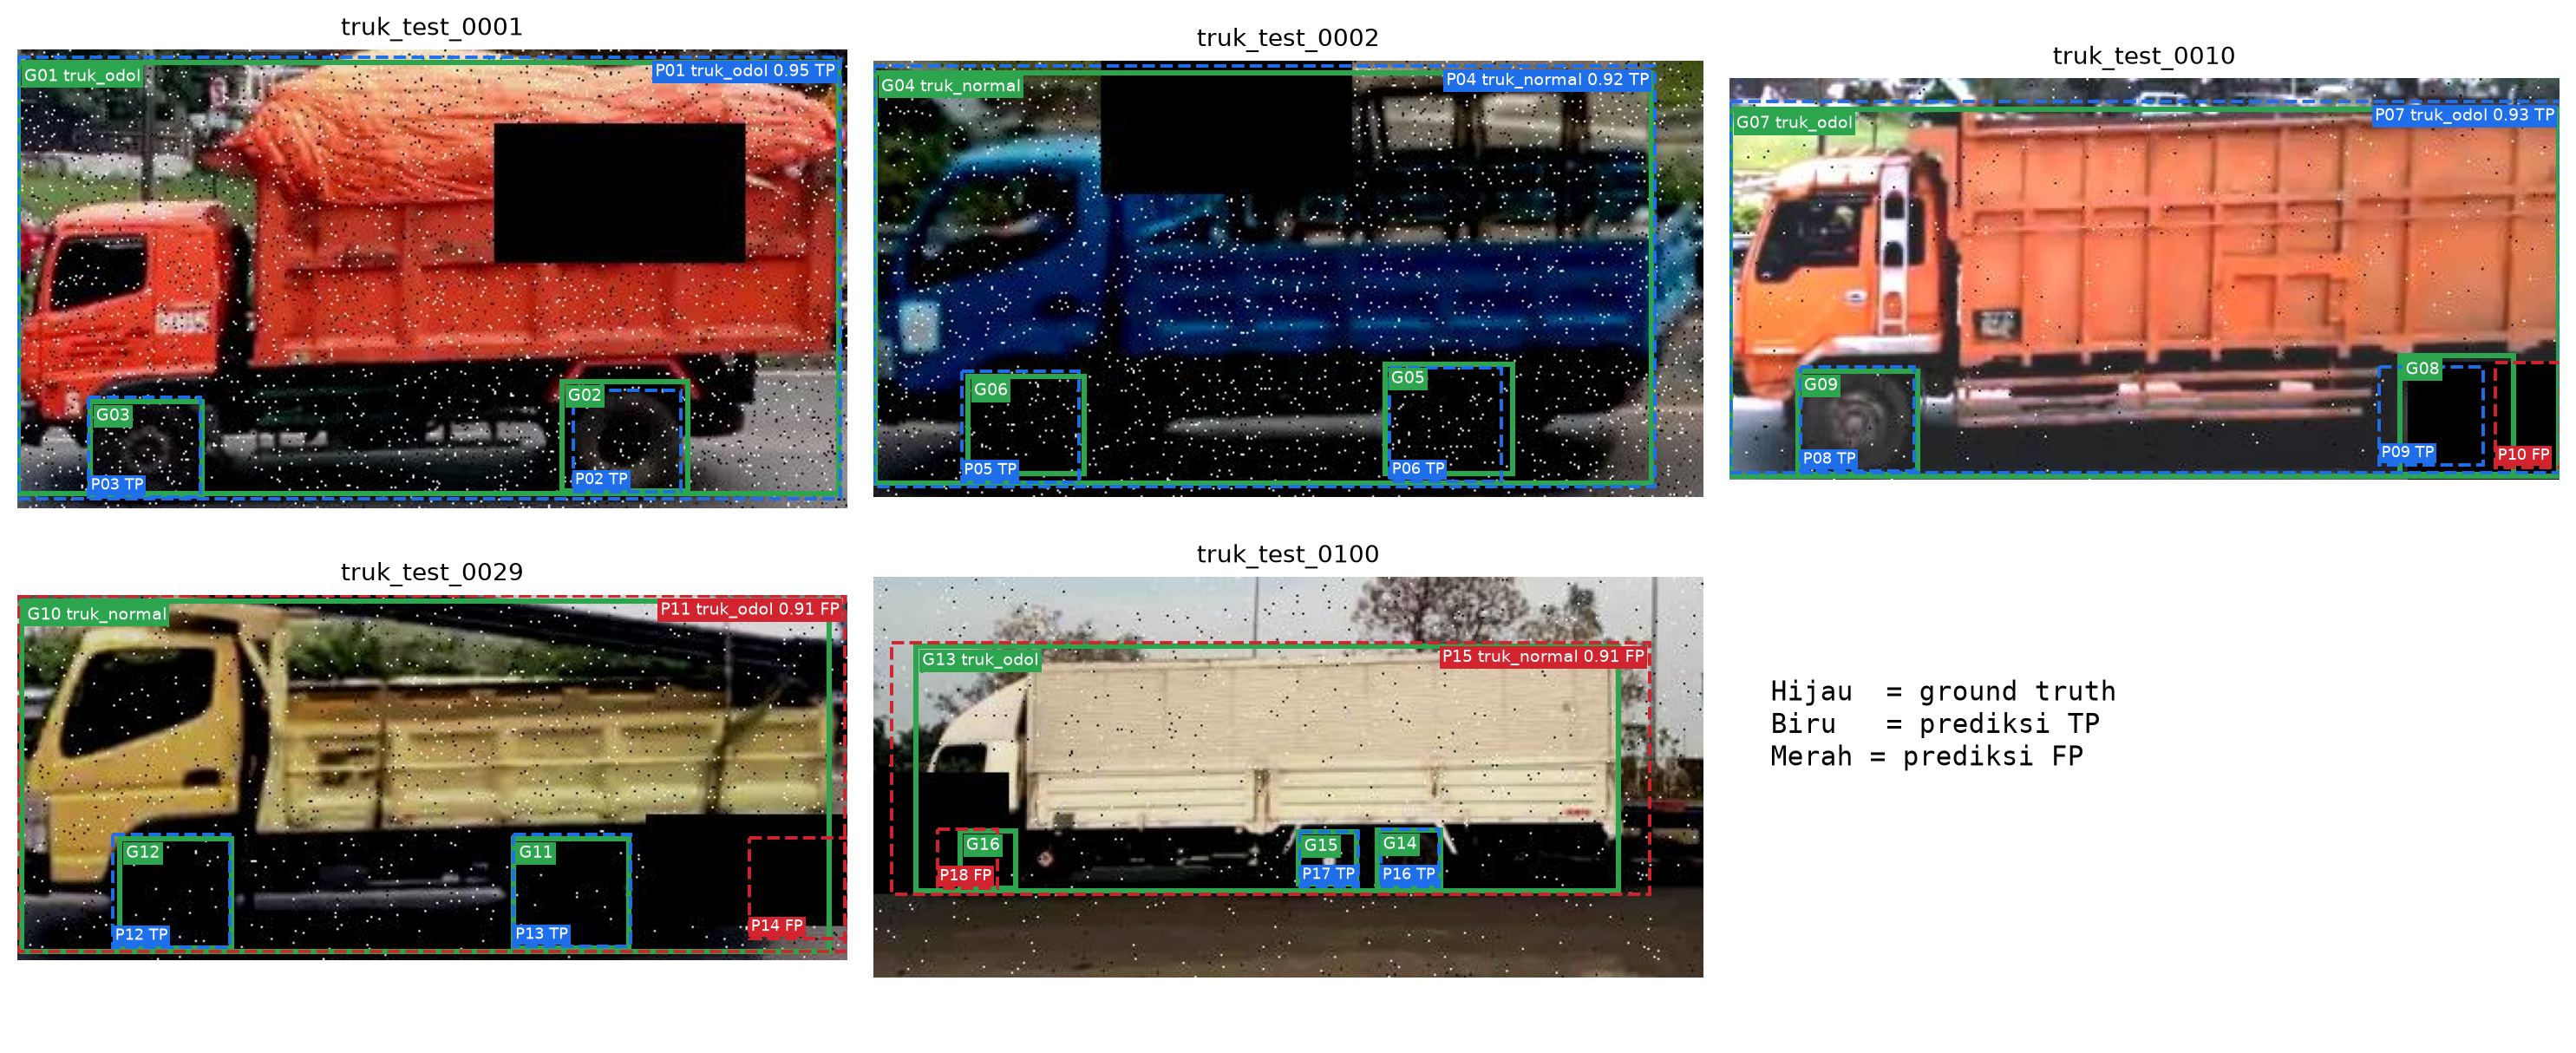
\includegraphics[width=\linewidth]{deteksi_gt_vs_prediksi.png}
\caption{Kotak GT (hijau), prediksi TP (biru), dan prediksi FP (merah) pada lima gambar uji. Label \kode{G..} adalah ID GT dan \kode{P..} adalah ID prediksi}
\label{fig:deteksi}
\end{figure}

\subsection{Intersection over Union (IoU)}
IoU mengukur seberapa rapat dua kotak bertumpang tindih:
\[
\symup{IoU} = \frac{\symup{luas\ irisan}}{\symup{luas}_A + \symup{luas}_B - \symup{luas\ irisan}}.
\]
Contoh untuk prediksi P09 (roda, gambar 0010) terhadap GT G08:
\begin{itemize}
\item kotak prediksi $(325{,}3;\ 144{,}1;\ 377{,}4;\ 193{,}2)$, luas $52{,}1 \times 49{,}1 = 2558{,}1$,
\item kotak GT $(335{,}5;\ 138{,}3;\ 392{,}5;\ 198{,}0)$, luas $57{,}0 \times 59{,}7 = 3402{,}9$,
\item irisan $(335{,}5;\ 144{,}1;\ 377{,}4;\ 193{,}2)$, luas $41{,}9 \times 49{,}1 = 2057{,}3$,
\item IoU $= 2057{,}3 / (2558{,}1 + 3402{,}9 - 2057{,}3) = 2057{,}3 / 3903{,}7 = 0{,}527$.
\end{itemize}
Karena $0{,}527 \geq 0{,}50$, P09 dihitung cocok.

\subsection{Pencocokan TP, FP, dan FN}
Prediksi diurutkan dari \textit{confidence} tertinggi. Sebuah prediksi menjadi TP jika IoU-nya $\geq 0{,}50$ terhadap GT berkelas sama yang belum dipakai; selain itu menjadi FP. GT yang tidak pernah cocok menjadi FN. Tabel~\ref{tab:match} hanya memuat kasus yang tidak sempurna; 13 prediksi lain adalah TP dengan IoU antara 0,53 dan 0,98.

\begin{table}[htbp]
\centering
\caption{Prediksi FP dan GT FN beserta penyebabnya. IoU dihitung terhadap GT terdekat dari kelas apa pun}
\label{tab:match}
\begin{grid}{width=\linewidth, colspec={Q[c,1.6cm] Q[c,0.9cm] Q[l,3.5cm] Q[c,1.3cm] Q[r,1cm] X[l]}, row{1}={halign=c}}
Gambar & ID & Kelas (conf.) & Status & IoU & Penyebab \\
0010 & P10 & roda (0,50)         & FP & 0,10 & Kotak kedua di sekitar roda kanan yang tertutup bidang hitam \\
0029 & P11 & truk\_odol (0,91)   & FP & 0,96 & Kotak tepat, kelas salah (GT \kode{truk\_normal}) \\
0029 & G10 & truk\_normal        & FN & --   & Terlewat karena diprediksi sebagai \kode{truk\_odol} \\
0029 & P14 & roda (0,43)         & FP & 0,03 & Roda palsu di area bidang hitam \\
0100 & P15 & truk\_normal (0,91) & FP & 0,90 & Kotak tepat, kelas salah (GT \kode{truk\_odol}) \\
0100 & G13 & truk\_odol          & FN & --   & Terlewat karena diprediksi sebagai \kode{truk\_normal} \\
0100 & P18 & roda (0,40)         & FP & 0,46 & Roda ditemukan, tetapi kotak bergeser sehingga IoU $< 0{,}50$ \\
0100 & G16 & roda                & FN & --   & Pasangan dari P18 \\
\end{grid}
\end{table}

\begin{table}[htbp]
\centering
\caption{Rekap TP, FP, FN, precision, dan recall per kelas (IoU $\geq 0{,}50$)}
\label{tab:rekapdet}
\begin{grid}{width=\linewidth, colspec={Q[l,2.7cm] Q[r,1cm] Q[r,1.8cm] Q[r,1cm] Q[r,1cm] Q[r,1cm] X[r] X[r]}, row{1}={halign=c}}
Kelas & GT & Prediksi & TP & FP & FN & Precision & Recall \\
roda         & 11 & 13 & 10 & 3 & 1 & 0,7692 & 0,9091 \\
truk\_normal & 2  & 2  & 1  & 1 & 1 & 0,5000 & 0,5000 \\
truk\_odol   & 3  & 3  & 2  & 1 & 1 & 0,6667 & 0,6667 \\
Semua kelas  & 16 & 18 & 13 & 5 & 3 & 0,7222 & 0,8125 \\
\end{grid}
\end{table}

\subsection{Average Precision (AP) dan mAP}
Untuk tiap kelas, prediksi diurutkan dari \textit{confidence} tertinggi lalu dihitung precision dan recall kumulatif. Precision kemudian diinterpolasi agar tidak naik dari kanan ke kiri, $p_{\symup{interp}}(r) = \max_{\tilde r \geq r} p(\tilde r)$, dan AP adalah luas di bawah kurva tersebut:
\[
\symup{AP} = \sum_n (r_n - r_{n-1})\, p_{\symup{interp}}(r_n).
\]

\begin{itemize}
\item \kode{roda} (11 GT): sepuluh prediksi teratas semuanya TP, sehingga precision tetap 1 sampai recall $10/11 = 0{,}909$. Tiga FP muncul paling akhir (\textit{confidence} $\leq 0{,}50$) dan tidak menambah recall. AP $= 0{,}909 \times 1 = 0{,}9091$.
\item \kode{truk\_normal} (2 GT): P04 TP (precision 1, recall 0,5), lalu P15 FP. AP $= 0{,}5 \times 1 = 0{,}5000$.
\item \kode{truk\_odol} (3 GT): P01 dan P07 TP (precision 1, recall 0,667), lalu P11 FP. AP $= 0{,}667 \times 1 = 0{,}6667$.
\end{itemize}
\[
\symup{mAP@0{,}50} = \frac{0{,}9091 + 0{,}5000 + 0{,}6667}{3} = 0{,}6919
\]

Sebagai verifikasi, fungsi \kode{ap\_per\_class} dari \kode{ultralytics} memakai interpolasi 101 titik dan menghasilkan mAP@0,50 $= 0{,}6883$. Selisih kecil ini berasal dari cara interpolasi, bukan dari kesalahan hitung. Sebagai pelengkap, mAP@0,50:0,95 (rata-rata pada ambang IoU 0,50 sampai 0,95) bernilai 0,5874 secara manual dan 0,5845 menurut \kode{ultralytics}.

\begin{figure}[htbp]
\centering
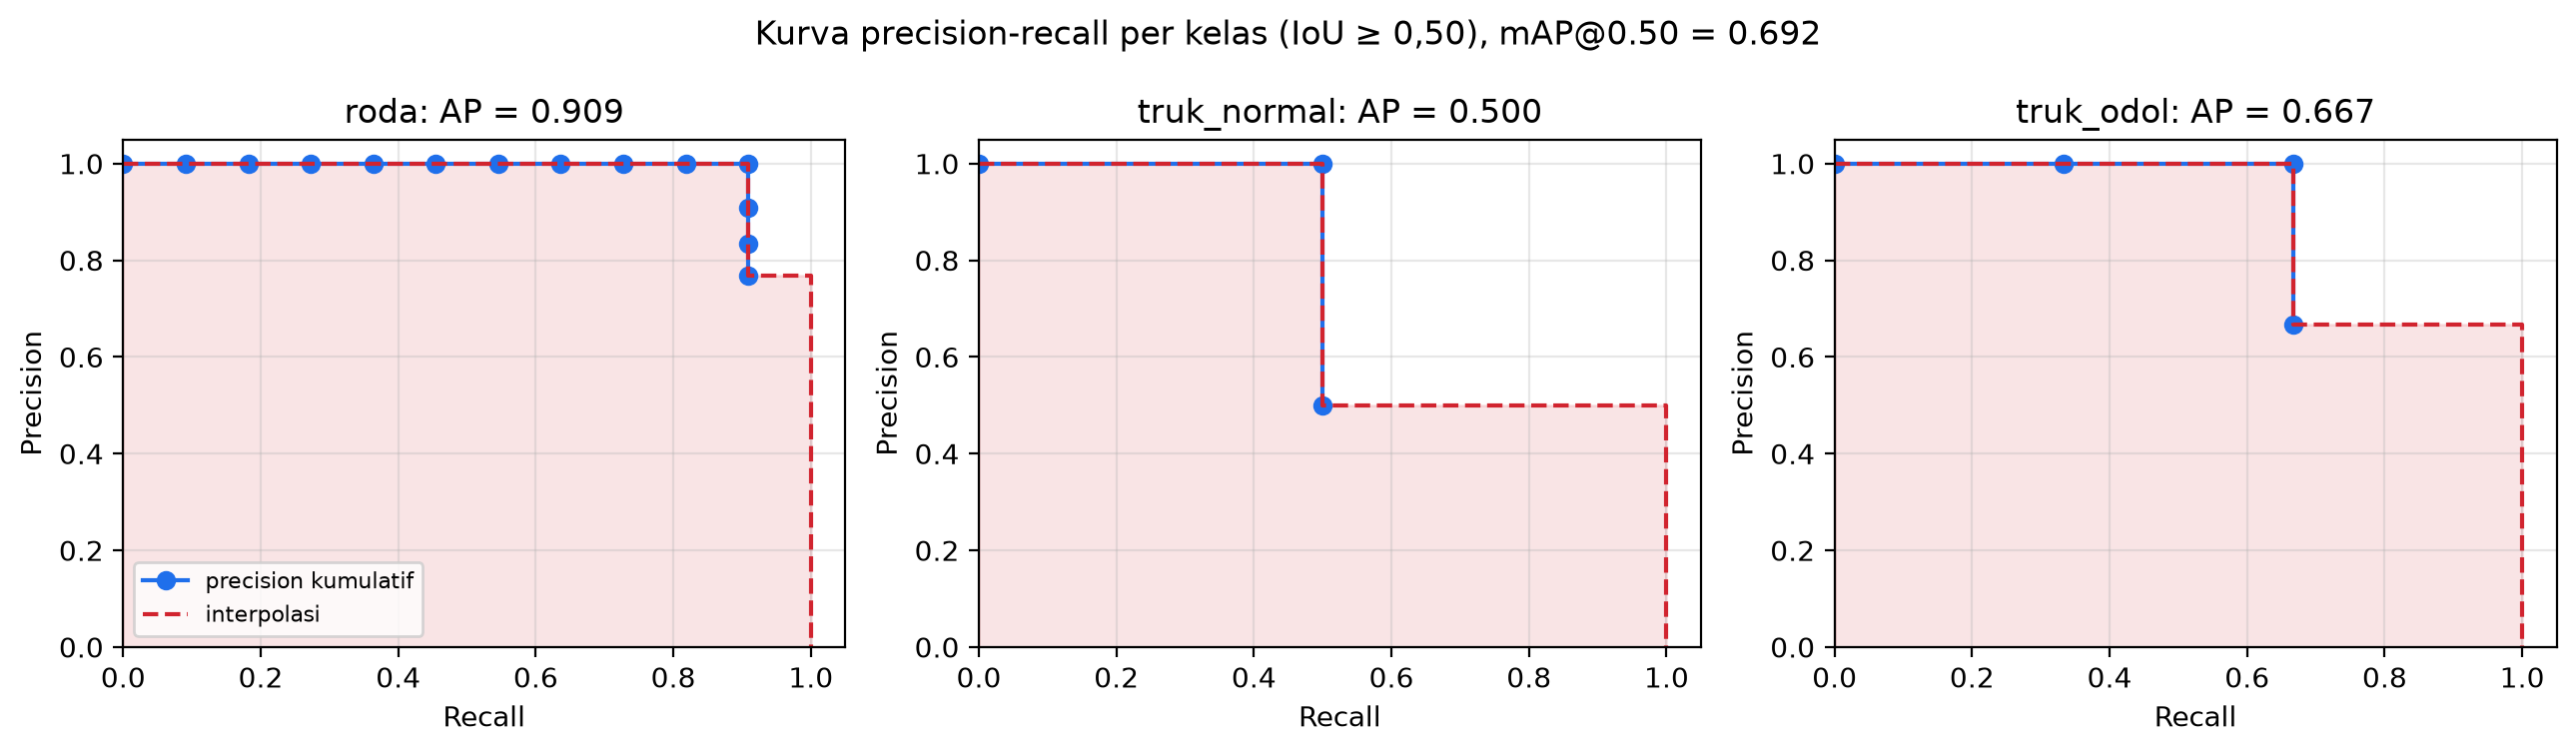
\includegraphics[width=\linewidth]{deteksi_kurva_pr.png}
\caption{Kurva precision-recall per kelas. Garis merah putus-putus adalah precision terinterpolasi; luas arsiran adalah AP}
\label{fig:pr}
\end{figure}

\subsection{Interpretasi}
\begin{itemize}
\item Gambar 0001 dan 0002 terdeteksi sempurna, dengan IoU semua pasangan di atas 0,78.
\item Kesalahan terbesar adalah tertukarnya kelas \kode{truk\_normal} dan \kode{truk\_odol} (gambar 0029 dan 0100). Lokalisasinya tepat (IoU 0,90 dan 0,96), tetapi setiap kasus menghasilkan satu FP sekaligus satu FN. Akibatnya AP kedua kelas truk jauh di bawah AP \kode{roda}.
\item Pada gambar 0100, roda paling kiri sebenarnya ditemukan, tetapi kotaknya bergeser sehingga IoU hanya 0,455. Ambang IoU membuat satu objek yang ditemukan tetap dihitung sebagai FP dan FN.
\item Pada gambar 0010, P09 hanya lolos tipis (IoU 0,527). Jika ambang dinaikkan ke 0,55, prediksi ini pun gagal; inilah alasan mAP@0,50:0,95 lebih rendah daripada mAP@0,50.
\item Untuk sistem penindakan ODOL, perbaikan paling berdampak adalah mengurangi kebingungan \kode{truk\_normal} dan \kode{truk\_odol}, misalnya dengan menambah data truk normal yang tampak mirip ODOL (bak tinggi, muatan penuh).
\end{itemize}

% ------------------------------------------------------------------ 6
\section{Ringkasan}

\begin{table}[htbp]
\centering
\caption{Ringkasan metrik keempat bagian}
\label{tab:ringkasan}
\begin{grid}{width=\linewidth, colspec={Q[l,3.6cm] Q[l,3.2cm] Q[r,2.4cm] X[l]}, row{1}={halign=c}}
Bagian & Metrik & Nilai & Catatan \\
\SetCell[r=4]{l} Regresi (WIM) & MAE  & 1,370 ton & rata-rata meleset 1,4 ton \\
& RMSE & 1,544 ton & ada beberapa error besar \\
& $R^2$ & 0,9714 & 97\% variasi dijelaskan \\
& MAPE & 6,09\% & WIM cenderung melebihkan (MPE $-1{,}48\%$) \\
\SetCell[r=3]{l} Clustering (k = 3) & Inertia & 952,50 & terbesar di cluster \textit{overload} \\
& Silhouette & 0,6294 & struktur jelas \\
& Davies-Bouldin & 0,4627 & kemiripan antarcluster rendah \\
\SetCell[r=3]{l} Klasifikasi 3 kelas & Accuracy & 0,7667 & dipengaruhi kelas mayoritas \\
& Macro $F_1$ & 0,7442 & lebih adil untuk data tidak seimbang \\
& Weighted $F_1$ & 0,7648 & \\
\SetCell[r=3]{l} Deteksi objek & Precision & 0,7222 & semua kelas, IoU $\geq 0{,}50$ \\
& Recall & 0,8125 & \\
& mAP@0,50 & 0,6919 & kelas truk tertukar \\
\end{grid}
\end{table}

Setiap jenis model membutuhkan metrik yang berbeda, dan satu angka saja tidak pernah cukup. Pada regresi, RMSE dan MPE menunjukkan hal yang tidak terlihat dari MAE. Pada clustering, metrik internal perlu dilengkapi validasi bisnis. Pada klasifikasi, accuracy bisa menipu ketika kelas tidak seimbang. Pada deteksi objek, kesalahan kelas dan kesalahan lokalisasi sama-sama menurunkan mAP.

\section*{Lampiran: Menjalankan Ulang Perhitungan}
Semua perhitungan dapat diulang dari folder \kode{kelompok-evaluasi-model}:
\begin{enumerate}
\item Pasang dependensi: \kode{pip install -r requirements.txt}.
\item Buka dan jalankan \kode{evaluasi\_model.ipynb}. Notebook membaca data dari folder \kode{data/} dan menyimpan gambar ke \kode{figures/}.
\item Prediksi deteksi objek sudah tersimpan di \kode{data/deteksi/prediksi\_yolo.csv}. Untuk membuatnya ulang dari model, jalankan:\newline \kode{python scripts/prediksi\_deteksi.py ../tugas/best.pt}
\end{enumerate}

\end{document}
